% 12 variables in here:
% u_1 = 3.9, h_1 = 11.0, U_1 = -1.3, H_1 = 11.3, u_2 = 1.7, h_2 = 8.6, U_2 = 3.5, H_2 = 11.9, u_3 = -3.2, h_3 = 11.4, U_3 = -3.8, H_3 = 8.7
\begin{figure}[h!t]
\centering
  \subfigure[Height and Impulse for point $p_1^L$] {
    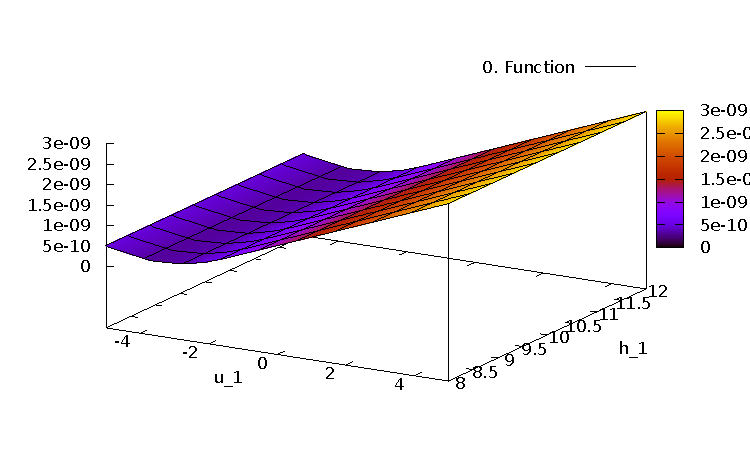
\includegraphics[scale=\zoomfactor]{{{3_random_new/x_y_-1.3_11.3_1.7_8.6_3.5_11.9_-3.2_11.4_-3.8_8.7f0}}}  
    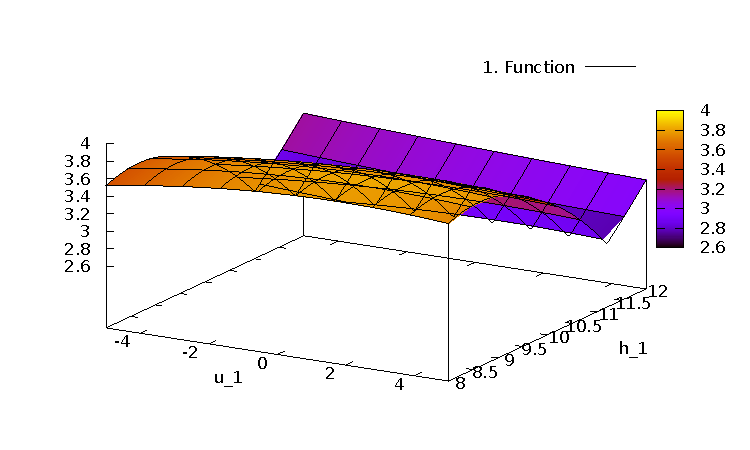
\includegraphics[scale=\zoomfactor]{{{3_random_new/x_y_-1.3_11.3_1.7_8.6_3.5_11.9_-3.2_11.4_-3.8_8.7f1}}}  
  }

  % \subfigure[Height and Impulse for point $p_2^L$] {
  %   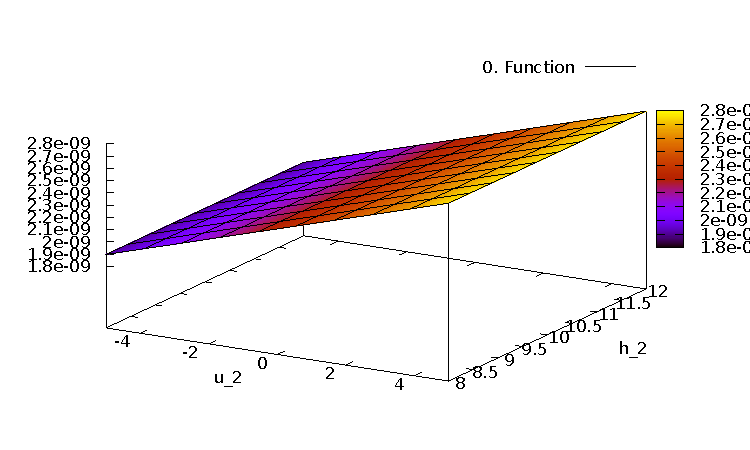
\includegraphics[scale=\zoomfactor]{{{3_random_new/3.9_11.0_-1.3_11.3_x_y_3.5_11.9_-3.2_11.4_-3.8_8.7f0}}}  
  %   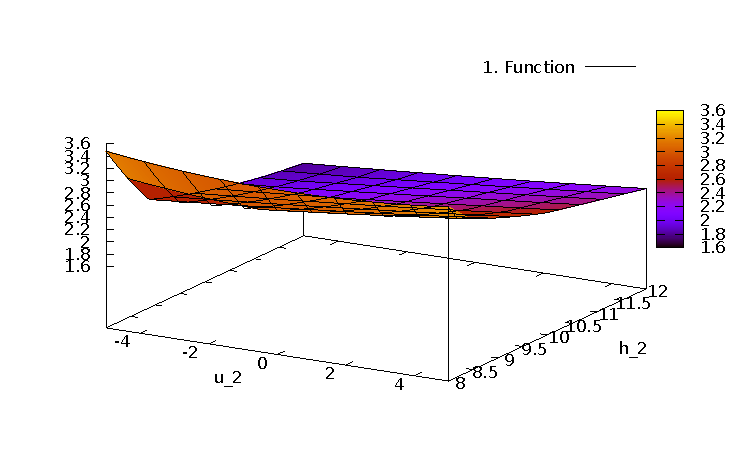
\includegraphics[scale=\zoomfactor]{{{3_random_new/3.9_11.0_-1.3_11.3_x_y_3.5_11.9_-3.2_11.4_-3.8_8.7f1}}}  
  % }

  \subfigure[Height and Impulse for point $p_3^L$] {
    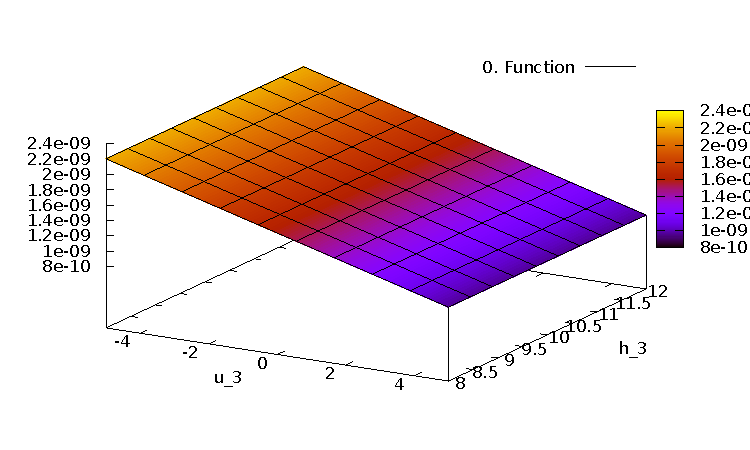
\includegraphics[scale=\zoomfactor]{{{3_random_new/3.9_11.0_-1.3_11.3_1.7_8.6_3.5_11.9_x_y_-3.8_8.7f0}}}  
    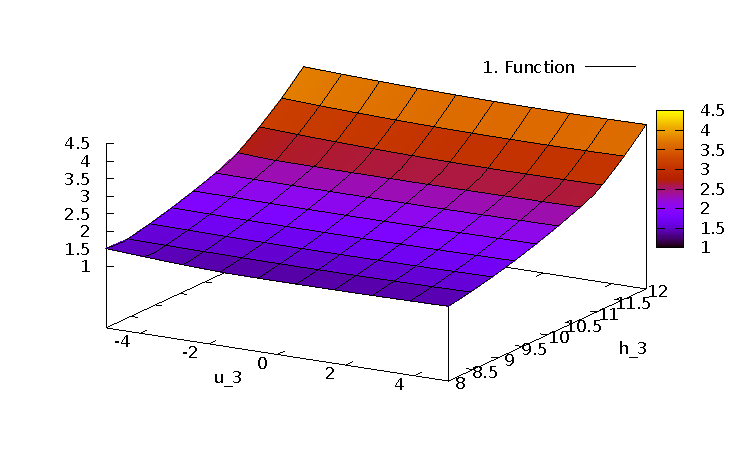
\includegraphics[scale=\zoomfactor]{{{3_random_new/3.9_11.0_-1.3_11.3_1.7_8.6_3.5_11.9_x_y_-3.8_8.7f1}}}  
  }

  \subfigure[Impulse for point $p_1^R$] {
    % 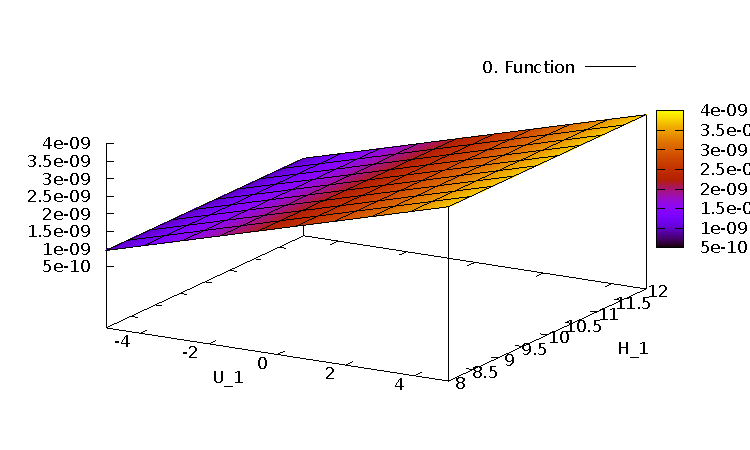
\includegraphics[scale=\zoomfactor]{{{3_random_new/3.9_11.0_x_y_1.7_8.6_3.5_11.9_-3.2_11.4_-3.8_8.7f0}}}  
    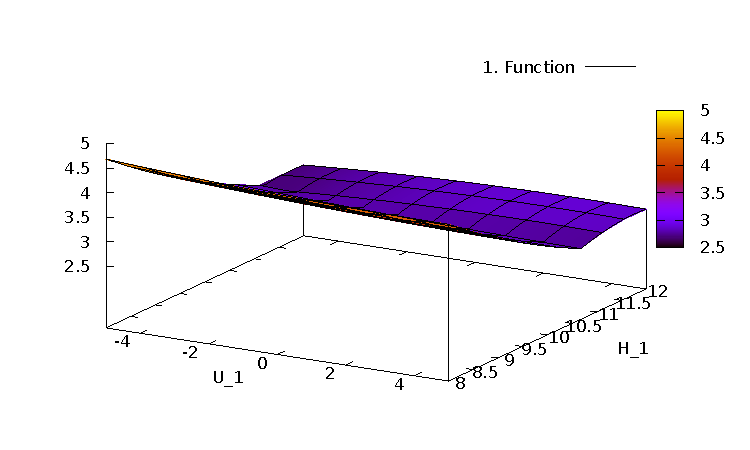
\includegraphics[scale=\zoomfactor]{{{3_random_new/3.9_11.0_x_y_1.7_8.6_3.5_11.9_-3.2_11.4_-3.8_8.7f1}}}  
  }
  \subfigure[Impulse for point $p_2^R$] {
    % 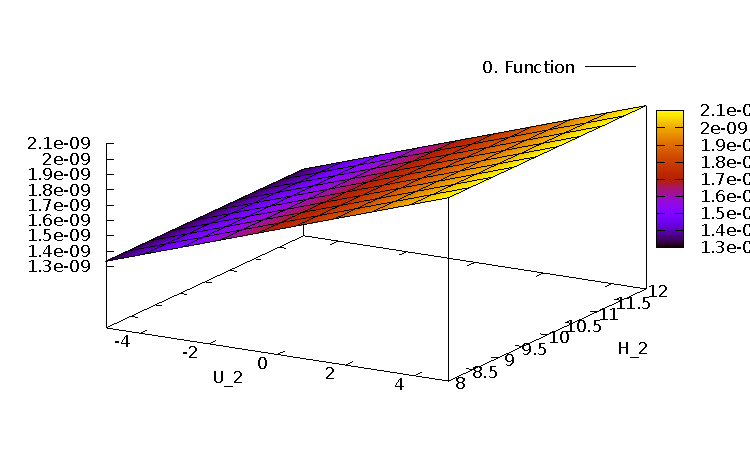
\includegraphics[scale=\zoomfactor]{{{3_random_new/3.9_11.0_-1.3_11.3_1.7_8.6_x_y_-3.2_11.4_-3.8_8.7f0}}}  
    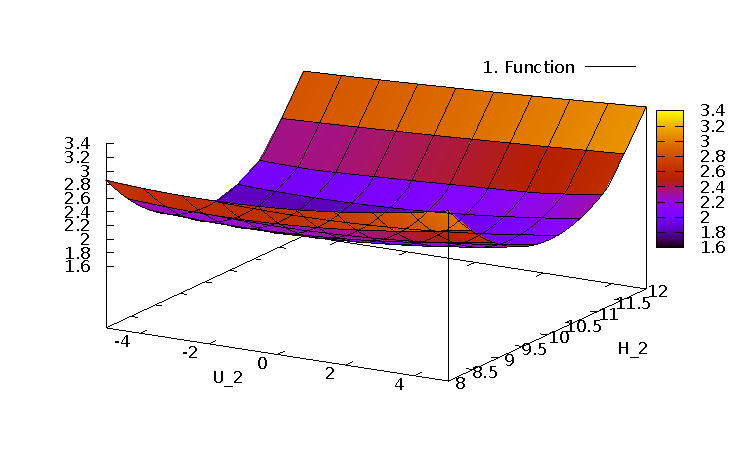
\includegraphics[scale=\zoomfactor]{{{3_random_new/3.9_11.0_-1.3_11.3_1.7_8.6_x_y_-3.2_11.4_-3.8_8.7f1}}}  
  }

  % \subfigure[Height and Impulse for point $p_3^R$] {
  %   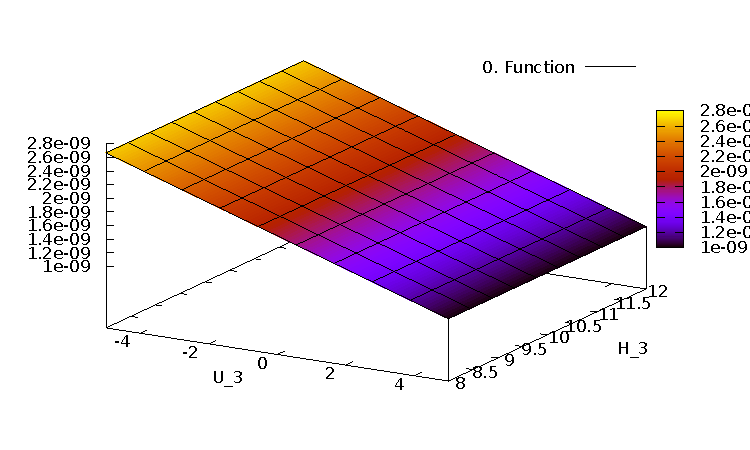
\includegraphics[scale=\zoomfactor]{{{3_random_new/3.9_11.0_-1.3_11.3_1.7_8.6_3.5_11.9_-3.2_11.4_x_yf0}}}  
  %   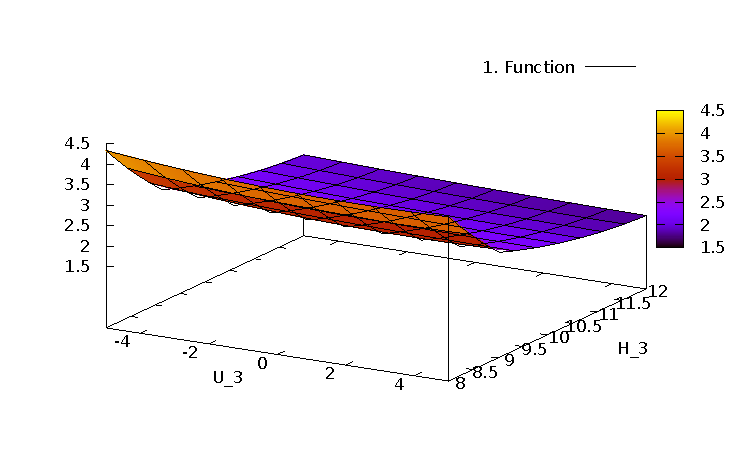
\includegraphics[scale=\zoomfactor]{{{3_random_new/3.9_11.0_-1.3_11.3_1.7_8.6_3.5_11.9_-3.2_11.4_x_yf1}}}  
  % }
\caption{Selected plots when choosing the height and impulse of three points randomly. Height and impulse data for these plots: $u_1^L = 3.9, h_1^L = 11.0, u_1^R = -1.3, h_1^R = 11.3, u_2^L = 1.7, h_2^L = 8.6, u_2^R = 3.5, h_2^R = 11.9, u_3^L = -3.2, h_3^L = 11.4, u_3^R = -3.8, h_3^R = 8.7$}
\label{fig:three-points-random}
\end{figure}

%%% Local Variables:
%%% TeX-master: "../results.tex"
%%% End: